\documentclass[a4paper,12pt]{article}
\usepackage{polski}
\usepackage[utf8]{inputenc}
\usepackage[OT4]{fontenc}
\usepackage{mathtools}
\usepackage{float}
\usepackage{graphicx}
\usepackage{multirow}

\newcommand{\h}[1]{\noindent \bf #1 \rm \\ \noindent}

\begin{document}

\begin{center}
	\LARGE
	Architektura Komputerów 2 \\
	\large
	WYKŁAD 1 
\end{center}
\vspace{1cm}
	
\h{Komputer:}
Komputer jest narzędziem, którego podstawowym zadaniem jest wykonywanie obliczeń. Jest to ponadto narzędzie zdolne wykonywać programy.\\

\h{Program:}
Programem nazywamy sformalizowany i utrwalony opis sposobu wykonywania działań, sekwencję operacji wykonywanych na strukturach danych. Program utrwalony być może na różne sposoby, chociażby na dysku twardym. \\

\begin{center}
	\it
	PROGRAM = ALGORYTMY + STRUKTURY DANYCH
\end{center}

\noindent
Program możemy opisać jako połączenie ustrukturyzowanych danych, na jakich dany program operuje oraz algorytmów, według których te dane są przetwarzane. \\

\h{Struktura danych:}
Strukturą danych nazywamy definicję danych i opis powiązań między nimi w logicznej przestrzeni adresowej. \\

\h{Algorytm:}
Algorytm to pewnego rodzaju formalny "przepis", ciąg operacji wykonywanych na danych. Składa się on z działań elementarnych, czyli instrukcji/rozkazów, które są zdefiniowane w architekturze komputera. \\

\newpage
\h{Architektura komputera a Organizacja komputera:}
\begin{table}[H]
	\centering
	\begin{tabular}{c|l}
		\hline
		\textbf{\begin{tabular}[c]{@{}c@{}}Architektura\\ Komputera\end{tabular}} & \begin{tabular}[c]{@{}l@{}}Specyfikacja funkcjonalnych cech komputera,\\ opisanych za pomocą listy rozkazów. Inaczej\\ nazywany architekturą listy rozkazów (ISA).\\ Opisuje interfejs programisty dla procesora.\end{tabular} \\ \hline
		\textbf{\begin{tabular}[c]{@{}c@{}}Organizacja\\ Komputera\end{tabular}}  & \begin{tabular}[c]{@{}l@{}}Architektura układów (HSA). Struktura logiczna \\ implementująca architekturę np. poprzez schemat\\ blokowy. Opisuje budowę i współdziałanie ele-\\ mentów procesora\end{tabular}                   \\ \hline
		\textbf{Realizacja}                                                       & \begin{tabular}[c]{@{}l@{}}Hardwear, który jest fizycznym zrealizowaniem\\ organizacji komputera.\end{tabular}                                                                                                                 \\ \hline
	\end{tabular}
\end{table}

\h{Maszyna Turinga:}
Model teoretyczny maszyny obliczeniowej, która składa się z:
\begin{itemize}
	\item Taśmy nieskończonej długości, podzielonej na pola, zawierające symbole.
	\item Głowicy odczytującej symbole z pól taśmy i wykonującej działania na podstawie odczytanych symboli oraz swojego aktualnego stanu.
\end{itemize}

\noindent
Maszyna Turinga jest de facto opisem komputera, gdzie:
\begin{itemize}
	\item Taśma jest pamięcią operacyjną procesora.
	\item Głowica jest procesorem.
	\item Stany głowicy są zawartością rejestrów procesora.
	\item Rozkazy maszyny są instrukcjami procesora.
\end{itemize}

\h{Architektura von Neumanna (Oksfordzka)}
Architektura, w której zarówno kody operacji jak i dane znajdują się na jednej taśmie (wspólnym obszarze pamięci).\\

\h{Architektura harwardzka:}
Modyfikacja modelu maszyny Turinga, w której zamiast jednej "taśmy" mamy dwie. Na jednej z nich znajduje się zapisany kod programu (kody operacji). Na drugiej zapisane są dane.\\

\noindent
Minusem takiego rozwiązania jest oczywiście zwiększony koszt, ze względu na wymóg posiadania 2 taśm, a co za tym idzie 2 głowic.\\

\noindent
Plusem architektury harwardzkiej jest możliwość zrównoleglenia operacji odczytu z obu taśm. Kolejną zaletą jest możliwość zabezpieczenia taśmy rozkazów przed zapisem (aby kod programu nie mógł zostać zmodyfikowany w trakcie jego wykonywania).\\

\h{Komputer z programem przechowywalnym:}
Komputer, w którym program jest zapamiętywany wewnątrz maszyny. Modelem teoretycznym, opisującym taki komputer jest maszyna Turinga. Procesor takiego komputera odczytuje/zapisuje dane z/do pamięci. Ponadto wykonuje polecenia po kolei z wyjątkiem wystąpienia operacji skoku do innego obszaru pamięci.\\

\begin{figure}[H]
	\centering
	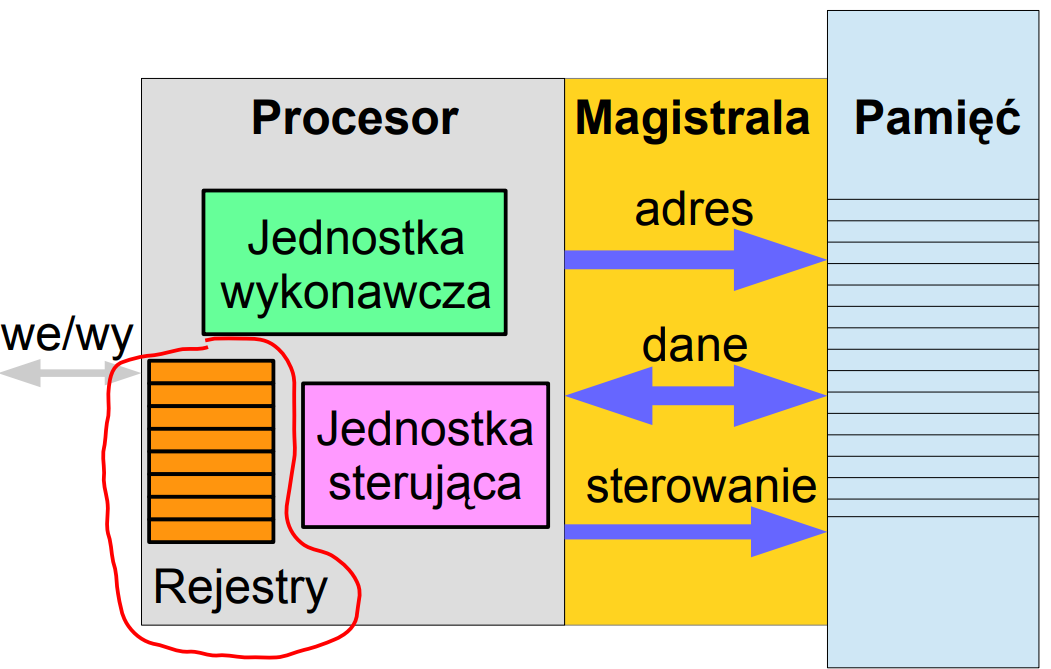
\includegraphics[width=10cm]{fig1.png}
	\caption{Schemat przedstawiający budowę komputera z programem przechowywalnym}
	\label{fig.budowa}
\end{figure}

\h{Magistrala:}
Magistrala jest elementem, który najbardziej wpływa na wydajność systemu (jej wydajność jest kilka tysięcy razy mniejsza od wydajności procesora). Jest to spowodowane relatywnie dużymi rozmiarami jak na standardy komputera (rząd centymetrów). To właśnie magistrala jest łącznikiem między pamięcią a procesorem. Właśnie przez to, że magistrala służy do komunikacji procesor-pamięć to jej rozmiary aż tak wpływają na jej wydajność.\\

\noindent
Magistrala to de facto wiązki przewodów. Dane są w niej reprezentowane i przesyłane w formie różnych wartości napięć na tychże przewodach. W magistrali mamy szyny z:
\begin{itemize}
	\item danymi
	\item adresami
	\item sterowaniem
\end{itemize}

\begin{figure}[H]
	\centering
	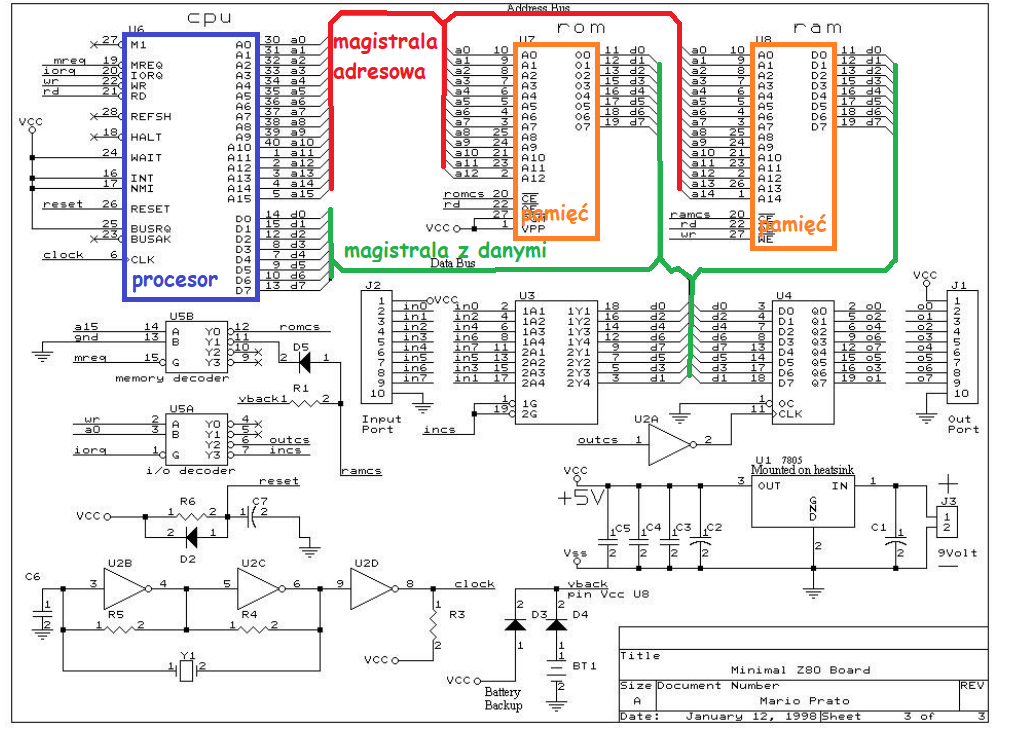
\includegraphics[width=12cm]{fig2.png}
	\caption{Schemat procesora Z80}
	\label{fig.magistrale}
\end{figure}

\h{Procesor:}
Procesor to składowa systemu składająca się z:
\begin{itemize}
	\item Od kilkunastu do kilkudziesięciu rejestrów zawierających dane o stanie procesora. 
	\item Jednostki wykonawczej wykonującej operacje arytmetyczne czy logiczne.
	\item Jednostki sterującej, najbardziej złożonej części CPU, która pobiera i interpretuje dane z taśmy i wydaje zlecenia jednostce wykonawczej. Jej działanie jest zależne od odczytanych danych oraz aktualnego stanu. Jego ona automatem.
\end{itemize}

\h{Pamięć:}
Ponumerowana tablica komórek (słów), czyli niepodzielnych kawałków pamięci. Każda komórka w pamięci ma ustalone miejsce w tablicy, które jest oznaczone przez wartość zwaną adresem. Pamięć n-bitowa to taka, składająca się z komórek o n-bitach. W takiej pamięci w jednym momencie można odczytać lub zapisać jednocześnie maksymalnie n-bitów.\\

\h{Typy pamięci (ze względu na architekturę):}
\begin{itemize}
	\item Pamięć RAM to pamięć o dostępie swobodnym (random access memory). Czyli pamięć składająca się z ponumerowanych komórek o jednakowym rozmiarze.  Jest ona relatywnie droga, gdyż na jej jeden przerzutnik przypada 1 bit zapamiętywanej informacji. Dostęp do danych jest w niej dosyć szybki. Po podaniu adresu od razu otrzymamy dostęp do odpowiadającej mu komórki.
	
	\item Pamięć SAM to pamięć o dostępie sekwencyjnym (sequential access memory). Czyli pamięć, w której czas dostępu do komórki zależy od tego jak bardzo jest ona oddalona od obecnego położenia w pamięci. W pamięci SAM komórki również mają przypisane adresy.
	
	\item Pamięć CAM to pamięć adresowana zawartością (content-addressable memory). Czyli pamięć, w której odnajdujemy dane na podstawie ich zawartości. Zadajemy pamięci jakiś wzorzec a ona zwraca nam adresy komórek które go spełniają. W związku z tym w celu wyszukania czegoś w takiej pamięci konieczne jest przeszukanie wszystkich jej komórek.
	
	\item Pamięć DDR(x), czyli hybryda RAM i SAM (double data rate), pozwalająca na przesył dwukrotnie większej ilości danych w jednym cyklu zegara niż starsze standardy. Tak szybka transmisja jest możliwa dzięki temu, że przesył następuje na dwóch zboczach sygnału zegarowego.
\end{itemize}

\h{Model programowy procesora (ISA):}
Model programowy procesora (Instruction Set Architecture). Definiuje aspekty procesora takie jak:
\begin{itemize}
	\item Lista rozkazów(instrukcje procesora)
	\item Tryby adresowania
	\item Rejestry - ich liczbę, rozmiary i przeznaczenie
	\item Typy danych
	\item Obsługę wyjątków i przerwań
\end{itemize}

\h{Proces tworzenia programu:}
\begin{enumerate}
	\item Tworzenie kodu źródłowego, czyli sposobu zapisu programu zrozumiałego dla człowieka.
	\item Przetworzenie kodu źródłowego przez kompilator do pliku obiektowego. Plik obiektowy zawiera kod maszynowy, zrozumiały dla komputera.
	\item Konsolidacja plików obiektowych w program przez konsolidator (linker). Uzyskanie programu wykonywalnego.
	\item Użycie programu ładującego do uruchomienia programu wykonywalnego na komputerze.
\end{enumerate}

\begin{figure}[H]
	\centering
	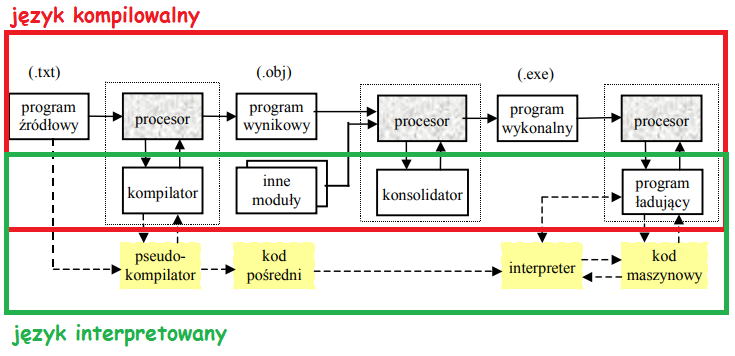
\includegraphics[width=15cm]{fig3.png}
	\caption{Schemat przedstawiający proces pisania programu.}
	\label{fig.proces.pisania.programu}
\end{figure}
	
\end{document}